\documentclass[1p]{elsarticle_modified}
%\bibliographystyle{elsarticle-num}

%\usepackage[colorlinks]{hyperref}
%\usepackage{abbrmath_seonhwa} %\Abb, \Ascr, \Acal ,\Abf, \Afrak
\usepackage{amsfonts}
\usepackage{amssymb}
\usepackage{amsmath}
\usepackage{amsthm}
\usepackage{scalefnt}
\usepackage{amsbsy}
\usepackage{kotex}
\usepackage{caption}
\usepackage{subfig}
\usepackage{color}
\usepackage{graphicx}
\usepackage{xcolor} %% white, black, red, green, blue, cyan, magenta, yellow
\usepackage{float}
\usepackage{setspace}
\usepackage{hyperref}

\usepackage{tikz}
\usetikzlibrary{arrows}

\usepackage{multirow}
\usepackage{array} % fixed length table
\usepackage{hhline}

%%%%%%%%%%%%%%%%%%%%%
\makeatletter
\renewcommand*\env@matrix[1][\arraystretch]{%
	\edef\arraystretch{#1}%
	\hskip -\arraycolsep
	\let\@ifnextchar\new@ifnextchar
	\array{*\c@MaxMatrixCols c}}
\makeatother %https://tex.stackexchange.com/questions/14071/how-can-i-increase-the-line-spacing-in-a-matrix
%%%%%%%%%%%%%%%

\usepackage[normalem]{ulem}

\newcommand{\msout}[1]{\ifmmode\text{\sout{\ensuremath{#1}}}\else\sout{#1}\fi}
%SOURCE: \msout is \stkout macro in https://tex.stackexchange.com/questions/20609/strikeout-in-math-mode

\newcommand{\cancel}[1]{
	\ifmmode
	{\color{red}\msout{#1}}
	\else
	{\color{red}\sout{#1}}
	\fi
}

\newcommand{\add}[1]{
	{\color{blue}\uwave{#1}}
}

\newcommand{\replace}[2]{
	\ifmmode
	{\color{red}\msout{#1}}{\color{blue}\uwave{#2}}
	\else
	{\color{red}\sout{#1}}{\color{blue}\uwave{#2}}
	\fi
}

\newcommand{\Sol}{\mathcal{S}} %segment
\newcommand{\D}{D} %diagram
\newcommand{\A}{\mathcal{A}} %arc


%%%%%%%%%%%%%%%%%%%%%%%%%%%%%5 test

\def\sl{\operatorname{\textup{SL}}(2,\Cbb)}
\def\psl{\operatorname{\textup{PSL}}(2,\Cbb)}
\def\quan{\mkern 1mu \triangleright \mkern 1mu}

\theoremstyle{definition}
\newtheorem{thm}{Theorem}[section]
\newtheorem{prop}[thm]{Proposition}
\newtheorem{lem}[thm]{Lemma}
\newtheorem{ques}[thm]{Question}
\newtheorem{cor}[thm]{Corollary}
\newtheorem{defn}[thm]{Definition}
\newtheorem{exam}[thm]{Example}
\newtheorem{rmk}[thm]{Remark}
\newtheorem{alg}[thm]{Algorithm}

\newcommand{\I}{\sqrt{-1}}
\begin{document}

%\begin{frontmatter}
%
%\title{Boundary parabolic representations of knots up to 8 crossings}
%
%%% Group authors per affiliation:
%\author{Yunhi Cho} 
%\address{Department of Mathematics, University of Seoul, Seoul, Korea}
%\ead{yhcho@uos.ac.kr}
%
%
%\author{Seonhwa Kim} %\fnref{s_kim}}
%\address{Center for Geometry and Physics, Institute for Basic Science, Pohang, 37673, Korea}
%\ead{ryeona17@ibs.re.kr}
%
%\author{Hyuk Kim}
%\address{Department of Mathematical Sciences, Seoul National University, Seoul 08826, Korea}
%\ead{hyukkim@snu.ac.kr}
%
%\author{Seokbeom Yoon}
%\address{Department of Mathematical Sciences, Seoul National University, Seoul, 08826,  Korea}
%\ead{sbyoon15@snu.ac.kr}
%
%\begin{abstract}
%We find all boundary parabolic representation of knots up to 8 crossings.
%
%\end{abstract}
%\begin{keyword}
%    \MSC[2010] 57M25 
%\end{keyword}
%
%\end{frontmatter}

%\linenumbers
%\tableofcontents
%
\newcommand\colored[1]{\textcolor{white}{\rule[-0.35ex]{0.8em}{1.4ex}}\kern-0.8em\color{red} #1}%
%\newcommand\colored[1]{\textcolor{white}{ #1}\kern-2.17ex	\textcolor{white}{ #1}\kern-1.81ex	\textcolor{white}{ #1}\kern-2.15ex\color{red}#1	}

{\Large $\underline{11n_{47}~(K11n_{47})}$}

\setlength{\tabcolsep}{10pt}
\renewcommand{\arraystretch}{1.6}
\vspace{1cm}\begin{tabular}{m{100pt}>{\centering\arraybackslash}m{274pt}}
\multirow{5}{120pt}{
	\centering
	\includegraphics[width=112pt]{../../../GIT/diagram.site/Diagrams/png/663_11n_47.png}\\
\ \ \ A knot diagram\footnotemark}&
\allowdisplaybreaks
\textbf{Linearized knot diagam} \\
\cline{2-2}
 &
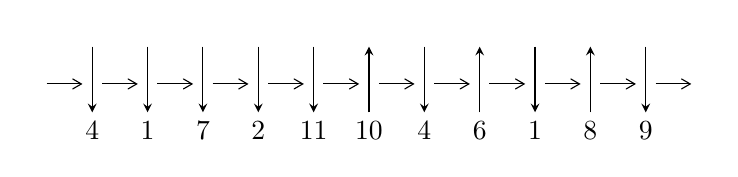
\begin{tikzpicture}[x=20pt, y=17pt]
	% nodes
	\node (C0) at (0, 0) {};
	\node (C1) at (1, 0) {};
	\node (C1U) at (1, +1) {};
	\node (C1D) at (1, -1) {4};

	\node (C2) at (2, 0) {};
	\node (C2U) at (2, +1) {};
	\node (C2D) at (2, -1) {1};

	\node (C3) at (3, 0) {};
	\node (C3U) at (3, +1) {};
	\node (C3D) at (3, -1) {7};

	\node (C4) at (4, 0) {};
	\node (C4U) at (4, +1) {};
	\node (C4D) at (4, -1) {2};

	\node (C5) at (5, 0) {};
	\node (C5U) at (5, +1) {};
	\node (C5D) at (5, -1) {11};

	\node (C6) at (6, 0) {};
	\node (C6U) at (6, +1) {};
	\node (C6D) at (6, -1) {10};

	\node (C7) at (7, 0) {};
	\node (C7U) at (7, +1) {};
	\node (C7D) at (7, -1) {4};

	\node (C8) at (8, 0) {};
	\node (C8U) at (8, +1) {};
	\node (C8D) at (8, -1) {6};

	\node (C9) at (9, 0) {};
	\node (C9U) at (9, +1) {};
	\node (C9D) at (9, -1) {1};

	\node (C10) at (10, 0) {};
	\node (C10U) at (10, +1) {};
	\node (C10D) at (10, -1) {8};

	\node (C11) at (11, 0) {};
	\node (C11U) at (11, +1) {};
	\node (C11D) at (11, -1) {9};
	\node (C12) at (12, 0) {};

	% arrows
	\draw[->,>={angle 60}]
	(C0) edge (C1) (C1) edge (C2) (C2) edge (C3) (C3) edge (C4) (C4) edge (C5) (C5) edge (C6) (C6) edge (C7) (C7) edge (C8) (C8) edge (C9) (C9) edge (C10) (C10) edge (C11) (C11) edge (C12) ;	\draw[->,>=stealth]
	(C1U) edge (C1D) (C2U) edge (C2D) (C3U) edge (C3D) (C4U) edge (C4D) (C5U) edge (C5D) (C6D) edge (C6U) (C7U) edge (C7D) (C8D) edge (C8U) (C9U) edge (C9D) (C10D) edge (C10U) (C11U) edge (C11D) ;
	\end{tikzpicture} \\
\hhline{~~} \\& 
\textbf{Solving Sequence} \\ \cline{2-2} 
 &
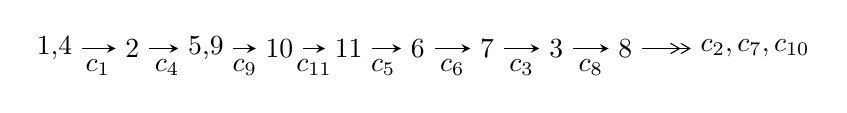
\begin{tikzpicture}[x=25pt, y=7pt]
	% node
	\node (A0) at (-1/8, 0) {1,4};
	\node (A1) at (1, 0) {2};
	\node (A2) at (33/16, 0) {5,9};
	\node (A3) at (25/8, 0) {10};
	\node (A4) at (33/8, 0) {11};
	\node (A5) at (41/8, 0) {6};
	\node (A6) at (49/8, 0) {7};
	\node (A7) at (57/8, 0) {3};
	\node (A8) at (65/8, 0) {8};
	\node (C1) at (1/2, -1) {$c_{1}$};
	\node (C2) at (3/2, -1) {$c_{4}$};
	\node (C3) at (21/8, -1) {$c_{9}$};
	\node (C4) at (29/8, -1) {$c_{11}$};
	\node (C5) at (37/8, -1) {$c_{5}$};
	\node (C6) at (45/8, -1) {$c_{6}$};
	\node (C7) at (53/8, -1) {$c_{3}$};
	\node (C8) at (61/8, -1) {$c_{8}$};
	\node (A9) at (10, 0) {$c_{2},c_{7},c_{10}$};

	% edge
	\draw[->,>=stealth]	
	(A0) edge (A1) (A1) edge (A2) (A2) edge (A3) (A3) edge (A4) (A4) edge (A5) (A5) edge (A6) (A6) edge (A7) (A7) edge (A8) ;
	\draw[->>,>={angle 60}]	
	(A8) edge (A9);
\end{tikzpicture} \\ 

\end{tabular} \\

\footnotetext{
The image of knot diagram is generated by the software ``\textbf{Draw programme}" developed by Andrew Bartholomew(\url{http://www.layer8.co.uk/maths/draw/index.htm\#Running-draw}), where we modified some parts for our purpose(\url{https://github.com/CATsTAILs/LinksPainter}).
}\phantom \\ \newline 
\centering \textbf{Ideals for irreducible components\footnotemark of $X_{\text{par}}$} 
 
\begin{align*}
I^u_{1}&=\langle 
7.57271\times10^{25} u^{34}+6.48827\times10^{26} u^{33}+\cdots+7.97336\times10^{26} b-7.26255\times10^{26},\\
\phantom{I^u_{1}}&\phantom{= \langle  }-1.64269\times10^{25} u^{34}-1.05850\times10^{26} u^{33}+\cdots+2.49168\times10^{25} a-1.38382\times10^{26},\;u^{35}+8 u^{34}+\cdots+9 u+1\rangle \\
I^u_{2}&=\langle 
b^6- b^5- b^4+2 b^3- b+1,\;a-1,\;u-1\rangle \\
I^u_{3}&=\langle 
b+1,\;2 u^2+a+4 u+4,\;u^3+u^2-1\rangle \\
\\
\end{align*}
\raggedright * 3 irreducible components of $\dim_{\mathbb{C}}=0$, with total 44 representations.\\
\footnotetext{All coefficients of polynomials are rational numbers. But the coefficients are sometimes approximated in decimal forms when there is not enough margin.}
\newpage
\renewcommand{\arraystretch}{1}
\centering \section*{I. $I^u_{1}= \langle 7.57\times10^{25} u^{34}+6.49\times10^{26} u^{33}+\cdots+7.97\times10^{26} b-7.26\times10^{26},\;-1.64\times10^{25} u^{34}-1.06\times10^{26} u^{33}+\cdots+2.49\times10^{25} a-1.38\times10^{26},\;u^{35}+8 u^{34}+\cdots+9 u+1 \rangle$}
\flushleft \textbf{(i) Arc colorings}\\
\begin{tabular}{m{7pt} m{180pt} m{7pt} m{180pt} }
\flushright $a_{1}=$&$\begin{pmatrix}1\\0\end{pmatrix}$ \\
\flushright $a_{4}=$&$\begin{pmatrix}0\\u\end{pmatrix}$ \\
\flushright $a_{2}=$&$\begin{pmatrix}1\\u^2\end{pmatrix}$ \\
\flushright $a_{5}=$&$\begin{pmatrix}- u\\- u^3+u\end{pmatrix}$ \\
\flushright $a_{9}=$&$\begin{pmatrix}0.659269 u^{34}+4.24813 u^{33}+\cdots+120.228 u+5.55377\\-0.0949751 u^{34}-0.813743 u^{33}+\cdots+1.09979 u+0.910851\end{pmatrix}$ \\
\flushright $a_{10}=$&$\begin{pmatrix}0.754244 u^{34}+5.06188 u^{33}+\cdots+119.128 u+4.64292\\-0.0949751 u^{34}-0.813743 u^{33}+\cdots+1.09979 u+0.910851\end{pmatrix}$ \\
\flushright $a_{11}=$&$\begin{pmatrix}-0.894280 u^{34}-6.14049 u^{33}+\cdots-123.987 u-2.97552\\-0.0130827 u^{34}-0.0126909 u^{33}+\cdots-5.06131 u-1.20991\end{pmatrix}$ \\
\flushright $a_{6}=$&$\begin{pmatrix}1.77774 u^{34}+17.8440 u^{33}+\cdots+23.8681 u-10.0326\\-0.414794 u^{34}-1.96166 u^{33}+\cdots+6.00083 u+0.386377\end{pmatrix}$ \\
\flushright $a_{7}=$&$\begin{pmatrix}0.135945 u^{34}+1.32830 u^{33}+\cdots+28.8699 u-0.0316372\\0.201606 u^{34}+1.17050 u^{33}+\cdots+2.73205 u+0.337551\end{pmatrix}$ \\
\flushright $a_{3}=$&$\begin{pmatrix}- u^2+1\\u^2\end{pmatrix}$ \\
\flushright $a_{8}=$&$\begin{pmatrix}0.135945 u^{34}+1.32830 u^{33}+\cdots+28.8699 u-0.0316372\\-0.239495 u^{34}-1.52839 u^{33}+\cdots+0.429444 u+0.0968115\end{pmatrix}$\\ \flushright $a_{8}=$&$\begin{pmatrix}0.135945 u^{34}+1.32830 u^{33}+\cdots+28.8699 u-0.0316372\\-0.239495 u^{34}-1.52839 u^{33}+\cdots+0.429444 u+0.0968115\end{pmatrix}$\\&\end{tabular}
\flushleft \textbf{(ii) Obstruction class $= -1$}\\~\\
\flushleft \textbf{(iii) Cusp Shapes $= -\frac{3378359165600571190629683677}{398668191729252960111215152} u^{34}-\frac{15526399702733176499705931937}{199334095864626480055607576} u^{33}+\cdots+\frac{65474135371669423713349877783}{398668191729252960111215152} u+\frac{2429897091838954454446349621}{199334095864626480055607576}$}\\~\\
\newpage\renewcommand{\arraystretch}{1}
\flushleft \textbf{(iv) u-Polynomials at the component}\newline \\
\begin{tabular}{m{50pt}|m{274pt}}
Crossings & \hspace{64pt}u-Polynomials at each crossing \\
\hline $$\begin{aligned}c_{1},c_{4}\end{aligned}$$&$\begin{aligned}
&u^{35}-8 u^{34}+\cdots+9 u-1
\end{aligned}$\\
\hline $$\begin{aligned}c_{2}\end{aligned}$$&$\begin{aligned}
&u^{35}+42 u^{34}+\cdots-129 u+1
\end{aligned}$\\
\hline $$\begin{aligned}c_{3},c_{7}\end{aligned}$$&$\begin{aligned}
&u^{35}+2 u^{34}+\cdots-320 u-64
\end{aligned}$\\
\hline $$\begin{aligned}c_{5}\end{aligned}$$&$\begin{aligned}
&u^{35}-8 u^{34}+\cdots+73 u+31
\end{aligned}$\\
\hline $$\begin{aligned}c_{6}\end{aligned}$$&$\begin{aligned}
&u^{35}-4 u^{34}+\cdots+1417 u+1219
\end{aligned}$\\
\hline $$\begin{aligned}c_{8}\end{aligned}$$&$\begin{aligned}
&u^{35}+3 u^{34}+\cdots+2 u+1
\end{aligned}$\\
\hline $$\begin{aligned}c_{9},c_{11}\end{aligned}$$&$\begin{aligned}
&u^{35}-5 u^{34}+\cdots+67 u-1
\end{aligned}$\\
\hline $$\begin{aligned}c_{10}\end{aligned}$$&$\begin{aligned}
&u^{35}+6 u^{34}+\cdots+124 u-8
\end{aligned}$\\
\hline
\end{tabular}\\~\\
\newpage\renewcommand{\arraystretch}{1}
\flushleft \textbf{(v) Riley Polynomials at the component}\newline \\
\begin{tabular}{m{50pt}|m{274pt}}
Crossings & \hspace{64pt}Riley Polynomials at each crossing \\
\hline $$\begin{aligned}c_{1},c_{4}\end{aligned}$$&$\begin{aligned}
&y^{35}-42 y^{34}+\cdots-129 y-1
\end{aligned}$\\
\hline $$\begin{aligned}c_{2}\end{aligned}$$&$\begin{aligned}
&y^{35}-90 y^{34}+\cdots+6323 y-1
\end{aligned}$\\
\hline $$\begin{aligned}c_{3},c_{7}\end{aligned}$$&$\begin{aligned}
&y^{35}-36 y^{34}+\cdots-20480 y-4096
\end{aligned}$\\
\hline $$\begin{aligned}c_{5}\end{aligned}$$&$\begin{aligned}
&y^{35}-52 y^{34}+\cdots+29509 y-961
\end{aligned}$\\
\hline $$\begin{aligned}c_{6}\end{aligned}$$&$\begin{aligned}
&y^{35}-4 y^{34}+\cdots+25178641 y-1485961
\end{aligned}$\\
\hline $$\begin{aligned}c_{8}\end{aligned}$$&$\begin{aligned}
&y^{35}+y^{34}+\cdots+14 y-1
\end{aligned}$\\
\hline $$\begin{aligned}c_{9},c_{11}\end{aligned}$$&$\begin{aligned}
&y^{35}-33 y^{34}+\cdots+5091 y-1
\end{aligned}$\\
\hline $$\begin{aligned}c_{10}\end{aligned}$$&$\begin{aligned}
&y^{35}+18 y^{34}+\cdots+7312 y-64
\end{aligned}$\\
\hline
\end{tabular}\\~\\
\newpage\flushleft \textbf{(vi) Complex Volumes and Cusp Shapes}
$$\begin{array}{c|c|c}  
\text{Solutions to }I^u_{1}& \I (\text{vol} + \sqrt{-1}CS) & \text{Cusp shape}\\
 \hline 
\begin{aligned}
u &= \phantom{-}0.964380 + 0.326022 I \\
a &= \phantom{-}0.35491 - 1.77356 I \\
b &= \phantom{-}1.401850 + 0.174541 I\end{aligned}
 & -4.47629 - 0.99972 I & -15.2464 + 0.4133 I \\ \hline\begin{aligned}
u &= \phantom{-}0.964380 - 0.326022 I \\
a &= \phantom{-}0.35491 + 1.77356 I \\
b &= \phantom{-}1.401850 - 0.174541 I\end{aligned}
 & -4.47629 + 0.99972 I & -15.2464 - 0.4133 I \\ \hline\begin{aligned}
u &= \phantom{-}0.679243 + 0.583622 I \\
a &= -0.155632 - 1.137360 I \\
b &= \phantom{-}0.397949 + 0.909235 I\end{aligned}
 & -1.63296 - 3.48211 I & -7.94104 + 7.54592 I \\ \hline\begin{aligned}
u &= \phantom{-}0.679243 - 0.583622 I \\
a &= -0.155632 + 1.137360 I \\
b &= \phantom{-}0.397949 - 0.909235 I\end{aligned}
 & -1.63296 + 3.48211 I & -7.94104 - 7.54592 I \\ \hline\begin{aligned}
u &= -0.990139 + 0.655507 I \\
a &= -0.886995 - 0.313990 I \\
b &= -0.934664 - 0.185167 I\end{aligned}
 & \phantom{-}1.54213 + 2.47872 I & \phantom{-0.000000 -}0. + 5.93000 I \\ \hline\begin{aligned}
u &= -0.990139 - 0.655507 I \\
a &= -0.886995 + 0.313990 I \\
b &= -0.934664 + 0.185167 I\end{aligned}
 & \phantom{-}1.54213 - 2.47872 I & \phantom{-0.000000 } 0. - 5.93000 I \\ \hline\begin{aligned}
u &= \phantom{-}1.204600 + 0.063415 I \\
a &= -0.412107 - 0.706810 I \\
b &= \phantom{-}0.628022 - 0.554154 I\end{aligned}
 & -3.08874 + 1.42303 I & -6.41632 - 5.79805 I \\ \hline\begin{aligned}
u &= \phantom{-}1.204600 - 0.063415 I \\
a &= -0.412107 + 0.706810 I \\
b &= \phantom{-}0.628022 + 0.554154 I\end{aligned}
 & -3.08874 - 1.42303 I & -6.41632 + 5.79805 I \\ \hline\begin{aligned}
u &= \phantom{-}0.779230\phantom{ +0.000000I} \\
a &= -1.08295\phantom{ +0.000000I} \\
b &= -0.0140385\phantom{ +0.000000I}\end{aligned}
 & -1.12597\phantom{ +0.000000I} & -9.35810\phantom{ +0.000000I} \\ \hline\begin{aligned}
u &= \phantom{-}0.605532 + 0.380104 I \\
a &= -1.67784 - 0.73020 I \\
b &= \phantom{-}0.361624 - 0.080090 I\end{aligned}
 & -1.46738 - 0.11420 I & -8.20214 + 0.34884 I\\
 \hline 
 \end{array}$$\newpage$$\begin{array}{c|c|c}  
\text{Solutions to }I^u_{1}& \I (\text{vol} + \sqrt{-1}CS) & \text{Cusp shape}\\
 \hline 
\begin{aligned}
u &= \phantom{-}0.605532 - 0.380104 I \\
a &= -1.67784 + 0.73020 I \\
b &= \phantom{-}0.361624 + 0.080090 I\end{aligned}
 & -1.46738 + 0.11420 I & -8.20214 - 0.34884 I \\ \hline\begin{aligned}
u &= \phantom{-}0.704998\phantom{ +0.000000I} \\
a &= \phantom{-}11.0900\phantom{ +0.000000I} \\
b &= \phantom{-}1.00991\phantom{ +0.000000I}\end{aligned}
 & -2.72892\phantom{ +0.000000I} & \phantom{-}194.390\phantom{ +0.000000I} \\ \hline\begin{aligned}
u &= -0.686181 + 0.154265 I \\
a &= -1.246620 - 0.427424 I \\
b &= -1.126280 - 0.497250 I\end{aligned}
 & -1.08296 - 5.42643 I & -0.21975 + 3.30530 I \\ \hline\begin{aligned}
u &= -0.686181 - 0.154265 I \\
a &= -1.246620 + 0.427424 I \\
b &= -1.126280 + 0.497250 I\end{aligned}
 & -1.08296 + 5.42643 I & -0.21975 - 3.30530 I \\ \hline\begin{aligned}
u &= \phantom{-}0.730316 + 1.119100 I \\
a &= -0.576099 + 0.700870 I \\
b &= -1.51689 - 0.33803 I\end{aligned}
 & -7.84770 - 8.00129 I & \phantom{-0.000000 } 0 \\ \hline\begin{aligned}
u &= \phantom{-}0.730316 - 1.119100 I \\
a &= -0.576099 - 0.700870 I \\
b &= -1.51689 + 0.33803 I\end{aligned}
 & -7.84770 + 8.00129 I & \phantom{-0.000000 } 0 \\ \hline\begin{aligned}
u &= \phantom{-}0.656190 + 1.188230 I \\
a &= -0.419118 + 0.434391 I \\
b &= -1.47252 + 0.05220 I\end{aligned}
 & -7.58070 + 0.56154 I & \phantom{-0.000000 } 0 \\ \hline\begin{aligned}
u &= \phantom{-}0.656190 - 1.188230 I \\
a &= -0.419118 - 0.434391 I \\
b &= -1.47252 - 0.05220 I\end{aligned}
 & -7.58070 - 0.56154 I & \phantom{-0.000000 } 0 \\ \hline\begin{aligned}
u &= -1.63022 + 0.11868 I \\
a &= \phantom{-}0.069536 + 0.327596 I \\
b &= \phantom{-}0.340175 - 0.686101 I\end{aligned}
 & -9.25057 + 1.88240 I & \phantom{-0.000000 } 0 \\ \hline\begin{aligned}
u &= -1.63022 - 0.11868 I \\
a &= \phantom{-}0.069536 - 0.327596 I \\
b &= \phantom{-}0.340175 + 0.686101 I\end{aligned}
 & -9.25057 - 1.88240 I & \phantom{-0.000000 } 0\\
 \hline 
 \end{array}$$\newpage$$\begin{array}{c|c|c}  
\text{Solutions to }I^u_{1}& \I (\text{vol} + \sqrt{-1}CS) & \text{Cusp shape}\\
 \hline 
\begin{aligned}
u &= -0.294421 + 0.137620 I \\
a &= -0.647696 - 1.089550 I \\
b &= -0.225869 - 0.594231 I\end{aligned}
 & \phantom{-}1.40601 + 1.20005 I & \phantom{-}2.74470 - 1.99044 I \\ \hline\begin{aligned}
u &= -0.294421 - 0.137620 I \\
a &= -0.647696 + 1.089550 I \\
b &= -0.225869 + 0.594231 I\end{aligned}
 & \phantom{-}1.40601 - 1.20005 I & \phantom{-}2.74470 + 1.99044 I \\ \hline\begin{aligned}
u &= -1.68600\phantom{ +0.000000I} \\
a &= \phantom{-}2.34569\phantom{ +0.000000I} \\
b &= \phantom{-}1.28757\phantom{ +0.000000I}\end{aligned}
 & -11.4779\phantom{ +0.000000I} & \phantom{-0.000000 } 0 \\ \hline\begin{aligned}
u &= -1.68299 + 0.18586 I \\
a &= \phantom{-}0.383087 - 0.343481 I \\
b &= \phantom{-}0.25892 - 1.52764 I\end{aligned}
 & -9.90660 + 6.51942 I & \phantom{-0.000000 } 0 \\ \hline\begin{aligned}
u &= -1.68299 - 0.18586 I \\
a &= \phantom{-}0.383087 + 0.343481 I \\
b &= \phantom{-}0.25892 + 1.52764 I\end{aligned}
 & -9.90660 - 6.51942 I & \phantom{-0.000000 } 0 \\ \hline\begin{aligned}
u &= -1.70107 + 0.39786 I \\
a &= -1.50913 - 0.63392 I \\
b &= -1.58042 + 0.58476 I\end{aligned}
 & -15.7071 + 13.7623 I & \phantom{-0.000000 } 0 \\ \hline\begin{aligned}
u &= -1.70107 - 0.39786 I \\
a &= -1.50913 + 0.63392 I \\
b &= -1.58042 - 0.58476 I\end{aligned}
 & -15.7071 - 13.7623 I & \phantom{-0.000000 } 0 \\ \hline\begin{aligned}
u &= \phantom{-}1.74717 + 0.03675 I \\
a &= -1.63248 + 0.11344 I \\
b &= -1.54159 + 0.19584 I\end{aligned}
 & -10.19430 + 4.27290 I & \phantom{-0.000000 } 0 \\ \hline\begin{aligned}
u &= \phantom{-}1.74717 - 0.03675 I \\
a &= -1.63248 - 0.11344 I \\
b &= -1.54159 - 0.19584 I\end{aligned}
 & -10.19430 - 4.27290 I & \phantom{-0.000000 } 0 \\ \hline\begin{aligned}
u &= -1.75068 + 0.06096 I \\
a &= \phantom{-}1.46330 + 0.02059 I \\
b &= \phantom{-}1.82396 - 0.77537 I\end{aligned}
 & -14.4753 + 2.5419 I & \phantom{-0.000000 } 0\\
 \hline 
 \end{array}$$\newpage$$\begin{array}{c|c|c}  
\text{Solutions to }I^u_{1}& \I (\text{vol} + \sqrt{-1}CS) & \text{Cusp shape}\\
 \hline 
\begin{aligned}
u &= -1.75068 - 0.06096 I \\
a &= \phantom{-}1.46330 - 0.02059 I \\
b &= \phantom{-}1.82396 + 0.77537 I\end{aligned}
 & -14.4753 - 2.5419 I & \phantom{-0.000000 } 0 \\ \hline\begin{aligned}
u &= -1.72022 + 0.43828 I \\
a &= -1.34465 - 0.58112 I \\
b &= -1.49438 + 0.29415 I\end{aligned}
 & -15.2163 + 5.6356 I & \phantom{-0.000000 } 0 \\ \hline\begin{aligned}
u &= -1.72022 - 0.43828 I \\
a &= -1.34465 + 0.58112 I \\
b &= -1.49438 - 0.29415 I\end{aligned}
 & -15.2163 - 5.6356 I & \phantom{-0.000000 } 0 \\ \hline\begin{aligned}
u &= -0.0306219 + 0.0974691 I \\
a &= -1.93881 + 9.66636 I \\
b &= \phantom{-}1.038380 + 0.224787 I\end{aligned}
 & -1.92040 - 0.80331 I & -4.44102 - 0.15082 I \\ \hline\begin{aligned}
u &= -0.0306219 - 0.0974691 I \\
a &= -1.93881 - 9.66636 I \\
b &= \phantom{-}1.038380 - 0.224787 I\end{aligned}
 & -1.92040 + 0.80331 I & -4.44102 + 0.15082 I\\
 \hline 
 \end{array}$$\newpage\newpage\renewcommand{\arraystretch}{1}
\centering \section*{II. $I^u_{2}= \langle b^6- b^5- b^4+2 b^3- b+1,\;a-1,\;u-1 \rangle$}
\flushleft \textbf{(i) Arc colorings}\\
\begin{tabular}{m{7pt} m{180pt} m{7pt} m{180pt} }
\flushright $a_{1}=$&$\begin{pmatrix}1\\0\end{pmatrix}$ \\
\flushright $a_{4}=$&$\begin{pmatrix}0\\1\end{pmatrix}$ \\
\flushright $a_{2}=$&$\begin{pmatrix}1\\1\end{pmatrix}$ \\
\flushright $a_{5}=$&$\begin{pmatrix}-1\\0\end{pmatrix}$ \\
\flushright $a_{9}=$&$\begin{pmatrix}1\\b\end{pmatrix}$ \\
\flushright $a_{10}=$&$\begin{pmatrix}- b+1\\b\end{pmatrix}$ \\
\flushright $a_{11}=$&$\begin{pmatrix}- b+1\\- b^2\end{pmatrix}$ \\
\flushright $a_{6}=$&$\begin{pmatrix}- b^3+b^2-1\\- b^4\end{pmatrix}$ \\
\flushright $a_{7}=$&$\begin{pmatrix}0\\b^5- b^4-2 b^3+b^2+b-1\end{pmatrix}$ \\
\flushright $a_{3}=$&$\begin{pmatrix}0\\1\end{pmatrix}$ \\
\flushright $a_{8}=$&$\begin{pmatrix}0\\b^5- b^4-2 b^3+b^2+b-1\end{pmatrix}$\\ \flushright $a_{8}=$&$\begin{pmatrix}0\\b^5- b^4-2 b^3+b^2+b-1\end{pmatrix}$\\&\end{tabular}
\flushleft \textbf{(ii) Obstruction class $= 1$}\\~\\
\flushleft \textbf{(iii) Cusp Shapes $= 3 b^5+b^4+b^3-2 b^2+3 b-7$}\\~\\
\newpage\renewcommand{\arraystretch}{1}
\flushleft \textbf{(iv) u-Polynomials at the component}\newline \\
\begin{tabular}{m{50pt}|m{274pt}}
Crossings & \hspace{64pt}u-Polynomials at each crossing \\
\hline $$\begin{aligned}c_{1}\end{aligned}$$&$\begin{aligned}
&(u-1)^6
\end{aligned}$\\
\hline $$\begin{aligned}c_{2},c_{4}\end{aligned}$$&$\begin{aligned}
&(u+1)^6
\end{aligned}$\\
\hline $$\begin{aligned}c_{3},c_{7}\end{aligned}$$&$\begin{aligned}
&u^6
\end{aligned}$\\
\hline $$\begin{aligned}c_{5},c_{8}\end{aligned}$$&$\begin{aligned}
&u^6-3 u^5+5 u^4-4 u^3+2 u^2- u+1
\end{aligned}$\\
\hline $$\begin{aligned}c_{6},c_{11}\end{aligned}$$&$\begin{aligned}
&u^6- u^5- u^4+2 u^3- u+1
\end{aligned}$\\
\hline $$\begin{aligned}c_{9},c_{10}\end{aligned}$$&$\begin{aligned}
&u^6+u^5- u^4-2 u^3+u+1
\end{aligned}$\\
\hline
\end{tabular}\\~\\
\newpage\renewcommand{\arraystretch}{1}
\flushleft \textbf{(v) Riley Polynomials at the component}\newline \\
\begin{tabular}{m{50pt}|m{274pt}}
Crossings & \hspace{64pt}Riley Polynomials at each crossing \\
\hline $$\begin{aligned}c_{1},c_{2},c_{4}\end{aligned}$$&$\begin{aligned}
&(y-1)^6
\end{aligned}$\\
\hline $$\begin{aligned}c_{3},c_{7}\end{aligned}$$&$\begin{aligned}
&y^6
\end{aligned}$\\
\hline $$\begin{aligned}c_{5},c_{8}\end{aligned}$$&$\begin{aligned}
&y^6+y^5+5 y^4+6 y^2+3 y+1
\end{aligned}$\\
\hline $$\begin{aligned}c_{6},c_{9},c_{10}\\c_{11}\end{aligned}$$&$\begin{aligned}
&y^6-3 y^5+5 y^4-4 y^3+2 y^2- y+1
\end{aligned}$\\
\hline
\end{tabular}\\~\\
\newpage\flushleft \textbf{(vi) Complex Volumes and Cusp Shapes}
$$\begin{array}{c|c|c}  
\text{Solutions to }I^u_{2}& \I (\text{vol} + \sqrt{-1}CS) & \text{Cusp shape}\\
 \hline 
\begin{aligned}
u &= \phantom{-}1.00000\phantom{ +0.000000I} \\
a &= \phantom{-}1.00000\phantom{ +0.000000I} \\
b &= -1.002190 + 0.295542 I\end{aligned}
 & -3.53554 + 0.92430 I & -12.60470 + 5.55069 I \\ \hline\begin{aligned}
u &= \phantom{-}1.00000\phantom{ +0.000000I} \\
a &= \phantom{-}1.00000\phantom{ +0.000000I} \\
b &= -1.002190 - 0.295542 I\end{aligned}
 & -3.53554 - 0.92430 I & -12.60470 - 5.55069 I \\ \hline\begin{aligned}
u &= \phantom{-}1.00000\phantom{ +0.000000I} \\
a &= \phantom{-}1.00000\phantom{ +0.000000I} \\
b &= \phantom{-}0.428243 + 0.664531 I\end{aligned}
 & \phantom{-}0.245672 + 0.924305 I & -5.68949 - 0.25702 I \\ \hline\begin{aligned}
u &= \phantom{-}1.00000\phantom{ +0.000000I} \\
a &= \phantom{-}1.00000\phantom{ +0.000000I} \\
b &= \phantom{-}0.428243 - 0.664531 I\end{aligned}
 & \phantom{-}0.245672 - 0.924305 I & -5.68949 + 0.25702 I \\ \hline\begin{aligned}
u &= \phantom{-}1.00000\phantom{ +0.000000I} \\
a &= \phantom{-}1.00000\phantom{ +0.000000I} \\
b &= \phantom{-}1.073950 + 0.558752 I\end{aligned}
 & -1.64493 - 5.69302 I & -11.7058 + 8.3306 I \\ \hline\begin{aligned}
u &= \phantom{-}1.00000\phantom{ +0.000000I} \\
a &= \phantom{-}1.00000\phantom{ +0.000000I} \\
b &= \phantom{-}1.073950 - 0.558752 I\end{aligned}
 & -1.64493 + 5.69302 I & -11.7058 - 8.3306 I\\
 \hline 
 \end{array}$$\newpage\newpage\renewcommand{\arraystretch}{1}
\centering \section*{III. $I^u_{3}= \langle b+1,\;2 u^2+a+4 u+4,\;u^3+u^2-1 \rangle$}
\flushleft \textbf{(i) Arc colorings}\\
\begin{tabular}{m{7pt} m{180pt} m{7pt} m{180pt} }
\flushright $a_{1}=$&$\begin{pmatrix}1\\0\end{pmatrix}$ \\
\flushright $a_{4}=$&$\begin{pmatrix}0\\u\end{pmatrix}$ \\
\flushright $a_{2}=$&$\begin{pmatrix}1\\u^2\end{pmatrix}$ \\
\flushright $a_{5}=$&$\begin{pmatrix}- u\\u^2+u-1\end{pmatrix}$ \\
\flushright $a_{9}=$&$\begin{pmatrix}-2 u^2-4 u-4\\-1\end{pmatrix}$ \\
\flushright $a_{10}=$&$\begin{pmatrix}-2 u^2-4 u-3\\-1\end{pmatrix}$ \\
\flushright $a_{11}=$&$\begin{pmatrix}-2 u^2-4 u-3\\-1\end{pmatrix}$ \\
\flushright $a_{6}=$&$\begin{pmatrix}-7 u^2-13 u-9\\- u-2\end{pmatrix}$ \\
\flushright $a_{7}=$&$\begin{pmatrix}- u\\u^2+u-1\end{pmatrix}$ \\
\flushright $a_{3}=$&$\begin{pmatrix}- u^2+1\\u^2\end{pmatrix}$ \\
\flushright $a_{8}=$&$\begin{pmatrix}- u\\2 u^2+u-2\end{pmatrix}$\\ \flushright $a_{8}=$&$\begin{pmatrix}- u\\2 u^2+u-2\end{pmatrix}$\\&\end{tabular}
\flushleft \textbf{(ii) Obstruction class $= 1$}\\~\\
\flushleft \textbf{(iii) Cusp Shapes $= -21 u^2-53 u-51$}\\~\\
\newpage\renewcommand{\arraystretch}{1}
\flushleft \textbf{(iv) u-Polynomials at the component}\newline \\
\begin{tabular}{m{50pt}|m{274pt}}
Crossings & \hspace{64pt}u-Polynomials at each crossing \\
\hline $$\begin{aligned}c_{1}\end{aligned}$$&$\begin{aligned}
&u^3+u^2-1
\end{aligned}$\\
\hline $$\begin{aligned}c_{2},c_{7}\end{aligned}$$&$\begin{aligned}
&u^3+u^2+2 u+1
\end{aligned}$\\
\hline $$\begin{aligned}c_{3}\end{aligned}$$&$\begin{aligned}
&u^3- u^2+2 u-1
\end{aligned}$\\
\hline $$\begin{aligned}c_{4}\end{aligned}$$&$\begin{aligned}
&u^3- u^2+1
\end{aligned}$\\
\hline $$\begin{aligned}c_{5},c_{6}\end{aligned}$$&$\begin{aligned}
&u^3-2 u^2-3 u-1
\end{aligned}$\\
\hline $$\begin{aligned}c_{8}\end{aligned}$$&$\begin{aligned}
&u^3-3 u^2+2 u+1
\end{aligned}$\\
\hline $$\begin{aligned}c_{9}\end{aligned}$$&$\begin{aligned}
&(u-1)^3
\end{aligned}$\\
\hline $$\begin{aligned}c_{10}\end{aligned}$$&$\begin{aligned}
&u^3
\end{aligned}$\\
\hline $$\begin{aligned}c_{11}\end{aligned}$$&$\begin{aligned}
&(u+1)^3
\end{aligned}$\\
\hline
\end{tabular}\\~\\
\newpage\renewcommand{\arraystretch}{1}
\flushleft \textbf{(v) Riley Polynomials at the component}\newline \\
\begin{tabular}{m{50pt}|m{274pt}}
Crossings & \hspace{64pt}Riley Polynomials at each crossing \\
\hline $$\begin{aligned}c_{1},c_{4}\end{aligned}$$&$\begin{aligned}
&y^3- y^2+2 y-1
\end{aligned}$\\
\hline $$\begin{aligned}c_{2},c_{3},c_{7}\end{aligned}$$&$\begin{aligned}
&y^3+3 y^2+2 y-1
\end{aligned}$\\
\hline $$\begin{aligned}c_{5},c_{6}\end{aligned}$$&$\begin{aligned}
&y^3-10 y^2+5 y-1
\end{aligned}$\\
\hline $$\begin{aligned}c_{8}\end{aligned}$$&$\begin{aligned}
&y^3-5 y^2+10 y-1
\end{aligned}$\\
\hline $$\begin{aligned}c_{9},c_{11}\end{aligned}$$&$\begin{aligned}
&(y-1)^3
\end{aligned}$\\
\hline $$\begin{aligned}c_{10}\end{aligned}$$&$\begin{aligned}
&y^3
\end{aligned}$\\
\hline
\end{tabular}\\~\\
\newpage\flushleft \textbf{(vi) Complex Volumes and Cusp Shapes}
$$\begin{array}{c|c|c}  
\text{Solutions to }I^u_{3}& \I (\text{vol} + \sqrt{-1}CS) & \text{Cusp shape}\\
 \hline 
\begin{aligned}
u &= -0.877439 + 0.744862 I \\
a &= -0.920404 - 0.365165 I \\
b &= -1.00000\phantom{ +0.000000I}\end{aligned}
 & \phantom{-}1.37919 + 2.82812 I & -9.0124 - 12.0277 I \\ \hline\begin{aligned}
u &= -0.877439 - 0.744862 I \\
a &= -0.920404 + 0.365165 I \\
b &= -1.00000\phantom{ +0.000000I}\end{aligned}
 & \phantom{-}1.37919 - 2.82812 I & -9.0124 + 12.0277 I \\ \hline\begin{aligned}
u &= \phantom{-}0.754878\phantom{ +0.000000I} \\
a &= -8.15919\phantom{ +0.000000I} \\
b &= -1.00000\phantom{ +0.000000I}\end{aligned}
 & -2.75839\phantom{ +0.000000I} & -102.980\phantom{ +0.000000I}\\
 \hline 
 \end{array}$$\newpage
\newpage\renewcommand{\arraystretch}{1}
\centering \section*{ IV. u-Polynomials}
\begin{tabular}{m{50pt}|m{274pt}}
Crossings & \hspace{64pt}u-Polynomials at each crossing \\
\hline $$\begin{aligned}c_{1}\end{aligned}$$&$\begin{aligned}
&((u-1)^6)(u^3+u^2-1)(u^{35}-8 u^{34}+\cdots+9 u-1)
\end{aligned}$\\
\hline $$\begin{aligned}c_{2}\end{aligned}$$&$\begin{aligned}
&((u+1)^6)(u^3+u^2+2 u+1)(u^{35}+42 u^{34}+\cdots-129 u+1)
\end{aligned}$\\
\hline $$\begin{aligned}c_{3}\end{aligned}$$&$\begin{aligned}
&u^6(u^3- u^2+2 u-1)(u^{35}+2 u^{34}+\cdots-320 u-64)
\end{aligned}$\\
\hline $$\begin{aligned}c_{4}\end{aligned}$$&$\begin{aligned}
&((u+1)^6)(u^3- u^2+1)(u^{35}-8 u^{34}+\cdots+9 u-1)
\end{aligned}$\\
\hline $$\begin{aligned}c_{5}\end{aligned}$$&$\begin{aligned}
&(u^3-2 u^2-3 u-1)(u^6-3 u^5+5 u^4-4 u^3+2 u^2- u+1)\\
&\cdot(u^{35}-8 u^{34}+\cdots+73 u+31)
\end{aligned}$\\
\hline $$\begin{aligned}c_{6}\end{aligned}$$&$\begin{aligned}
&(u^3-2 u^2-3 u-1)(u^6- u^5- u^4+2 u^3- u+1)\\
&\cdot(u^{35}-4 u^{34}+\cdots+1417 u+1219)
\end{aligned}$\\
\hline $$\begin{aligned}c_{7}\end{aligned}$$&$\begin{aligned}
&u^6(u^3+u^2+2 u+1)(u^{35}+2 u^{34}+\cdots-320 u-64)
\end{aligned}$\\
\hline $$\begin{aligned}c_{8}\end{aligned}$$&$\begin{aligned}
&(u^3-3 u^2+2 u+1)(u^6-3 u^5+5 u^4-4 u^3+2 u^2- u+1)\\
&\cdot(u^{35}+3 u^{34}+\cdots+2 u+1)
\end{aligned}$\\
\hline $$\begin{aligned}c_{9}\end{aligned}$$&$\begin{aligned}
&((u-1)^3)(u^6+u^5+\cdots+u+1)(u^{35}-5 u^{34}+\cdots+67 u-1)
\end{aligned}$\\
\hline $$\begin{aligned}c_{10}\end{aligned}$$&$\begin{aligned}
&u^3(u^6+u^5+\cdots+u+1)(u^{35}+6 u^{34}+\cdots+124 u-8)
\end{aligned}$\\
\hline $$\begin{aligned}c_{11}\end{aligned}$$&$\begin{aligned}
&((u+1)^3)(u^6- u^5+\cdots- u+1)(u^{35}-5 u^{34}+\cdots+67 u-1)
\end{aligned}$\\
\hline
\end{tabular}\newpage\renewcommand{\arraystretch}{1}
\centering \section*{ V. Riley Polynomials}
\begin{tabular}{m{50pt}|m{274pt}}
Crossings & \hspace{64pt}Riley Polynomials at each crossing \\
\hline $$\begin{aligned}c_{1},c_{4}\end{aligned}$$&$\begin{aligned}
&((y-1)^6)(y^3- y^2+2 y-1)(y^{35}-42 y^{34}+\cdots-129 y-1)
\end{aligned}$\\
\hline $$\begin{aligned}c_{2}\end{aligned}$$&$\begin{aligned}
&((y-1)^6)(y^3+3 y^2+2 y-1)(y^{35}-90 y^{34}+\cdots+6323 y-1)
\end{aligned}$\\
\hline $$\begin{aligned}c_{3},c_{7}\end{aligned}$$&$\begin{aligned}
&y^6(y^3+3 y^2+2 y-1)(y^{35}-36 y^{34}+\cdots-20480 y-4096)
\end{aligned}$\\
\hline $$\begin{aligned}c_{5}\end{aligned}$$&$\begin{aligned}
&(y^3-10 y^2+5 y-1)(y^6+y^5+5 y^4+6 y^2+3 y+1)\\
&\cdot(y^{35}-52 y^{34}+\cdots+29509 y-961)
\end{aligned}$\\
\hline $$\begin{aligned}c_{6}\end{aligned}$$&$\begin{aligned}
&(y^3-10 y^2+5 y-1)(y^6-3 y^5+5 y^4-4 y^3+2 y^2- y+1)\\
&\cdot(y^{35}-4 y^{34}+\cdots+25178641 y-1485961)
\end{aligned}$\\
\hline $$\begin{aligned}c_{8}\end{aligned}$$&$\begin{aligned}
&(y^3-5 y^2+10 y-1)(y^6+y^5+5 y^4+6 y^2+3 y+1)\\
&\cdot(y^{35}+y^{34}+\cdots+14 y-1)
\end{aligned}$\\
\hline $$\begin{aligned}c_{9},c_{11}\end{aligned}$$&$\begin{aligned}
&(y-1)^3(y^6-3 y^5+5 y^4-4 y^3+2 y^2- y+1)\\
&\cdot(y^{35}-33 y^{34}+\cdots+5091 y-1)
\end{aligned}$\\
\hline $$\begin{aligned}c_{10}\end{aligned}$$&$\begin{aligned}
&y^3(y^6-3 y^5+\cdots- y+1)(y^{35}+18 y^{34}+\cdots+7312 y-64)
\end{aligned}$\\
\hline
\end{tabular}
\vskip 2pc
\end{document}